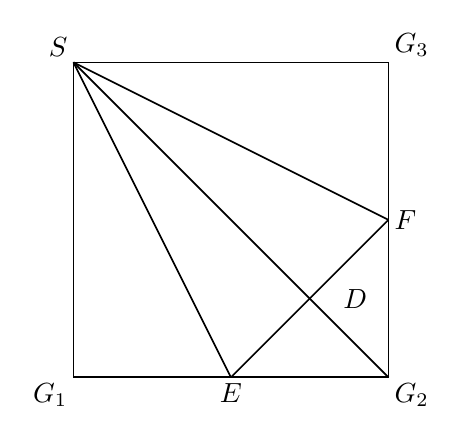
\begin{tikzpicture}[x=1cm,y=1cm,font=\normalsize,
 geometry edge/.style={solid,line width=.6pt},
 geometry mark/.style={solid,line width=.6pt},
 geometry label/.style={font=\normalsize,inner sep=2pt}]
\coordinate (S) at (0,4);
\coordinate (G3) at (4,4);
\coordinate (G2) at (4,0);
\coordinate (G1) at (0,0);
\coordinate (E) at (2,0);
\coordinate (F) at (4,2);
\coordinate (D) at (3,1);
\draw[geometry edge] (S)--(G3)--(G2)--(G1)--cycle;
\draw[geometry edge] (S)--(E);
\draw[geometry edge] (S)--(D);
\draw[geometry edge] (D)--(G2);
\draw[geometry edge] (S)--(F);
\draw[geometry edge] (E)--(D);
\draw[geometry edge] (D)--(F);
\node[geometry label,above left] at (S) {$S$};
\node[geometry label,above right] at (G3) {$G_3$};
\node[geometry label,below right] at (G2) {$G_2$};
\node[geometry label,below left] at (G1) {$G_1$};
\node[geometry label,below] at (E) {$E$};
\node[geometry label,right] at (F) {$F$};
\node[geometry label,right,xshift=10pt] at (D) {$D$};
\end{tikzpicture}